%! Author = jaroslav
%! Date = 17.04.20
\chapter{Глава третья}
\section{Часть третья}

Ранее был рассмотрен эксперимент с дилеммой заключенного и его сформулированный эффект.
Этот эффект хорошо моделируется с помощью квантово-подобных моделей принятия решений, благодаря
тому, что неопределенность описывется квантовой суперпозицией с точки зрения одного из игроков.
Таким образом описание неопределенности для игрока А относительно игрока Б описывается следующим образом:
\begin{equation}\label{phi_B}
    \vert \phi_{B} \rangle = \alpha \vert 0_{B} \rangle + \beta \vert 1_{B} \rangle \in \mathbb{C}^{2} % \mathbf{C}^{2}
\end{equation}
где $\alpha$ и $\beta$ - показывают степень осознания действия игрока Б, $\vert 0_{B} \rangle$ - характеризует
вектор предательства игроком Б, $\vert 1_{B} \rangle$ - характеризует вектор сотрудничества игроком Б.
$\mathbb{C}^{2}$ - двумерное комплексное пространство (в данном случае Гильбертово).
Для описания ситуации с учетом принятия решения игрока А, необходимо использовать четырехмерное Гильбертово
пространство $\mathbb{C}^{2} \otimes \mathbb{C}^{2}$.
В таком случае уравнение \eqref{phi_B} имеет следующий вид, в случае предательства игрока А~\citep{asano2011quantum}:
\begin{equation}
    \vert \Phi_{0_{A}} \rangle = \alpha_{0} \vert 0_{A} 0_{B} \rangle + \beta_{0} \vert 0_{A} 1_{B} \rangle \in \mathbb{C}^{2} \otimes \mathbb{C}^{2}
\end{equation}
С учетом сотрудничества игрока А, вектор общего психического состояния системы двух игроков записывается
следующим образом:
\begin{equation}
    \vert \Psi \rangle = \sum_{x,y=0}^{1} \alpha_{x,y} \vert x_{A} y_{B} \rangle =
    \alpha_{0} \vert 0_{A} 0_{B} \rangle + \beta_{0} \vert 0_{A} 1_{B} \rangle +
    \alpha_{1} \vert 1_{A} 0_{B} \rangle + \beta_{1} \vert 1_{A} 1_{B} \rangle
\end{equation}

Этот подход для описания состояния двух игроков позволяет рассматривать проблему на коллективном уровне.
Так например можно применить теорию открытых квантовых систем и рассматривать игрока А как квантовую
систему, а игрока Б как резервуар~\citep{bagarello2015operator,bagarello2015quantum}.
В этом случае игрока А будем обозначать как Алиса или агент $a$, а игрока Б как резервуар $b$.
В квантовой теории поля применима процедура квантования, основанная на алгебре операторов рождения
и уничтожения $a, a^{\dagger}, b, b^{\dagger}$.
Эти операторы позволяют рассматривать переход из одного квантового состояния в другое.
\begin{equation}
    \vert 1_{A} 0_{B} \rangle = a^{\dagger} \vert 0_{A} 0_{B} \rangle,
    \vert 0_{A} 1_{B} \rangle = a b^{\dagger} \vert 1_{A} 0_{B} \rangle
\end{equation}
Для данных операторов действуют следующие коммутационные соотношения:
\begin{equation}\label{CCR}
    [ a, a^{\dagger} ] = 1,
    [ b(k), b^{\dagger}(k) ] = \delta (k-k')
\end{equation}
где $k$ - размернность резервуара, $[x,y] = xy - yx$ - коммутатор.
Зная коммутационное соотношение~\eqref{CCR}, можно определить числовой оператор $n_a=a^{\dagger}a$
для агента.
Собственное значение этого оператора соответствует выбору, которым оперирует агент~\citep{bagarello2015quantum}.
Для определения операторов агента и резервуара используется уравнение Гейзенберга, которое имеет вид:
\begin{equation}
    i \hbar \frac{\partial f}{\partial t} = [f, H]
\end{equation}
где $i$ - мнимая единица, $\hbar$ - постоянная Планка, $\frac{\partial f}{\partial t}$ - дифференциал
функции $f$ по времени $t$, $[\cdot, \cdot]$ - коммутатор, $H$ - гамильтониан.
Для решения этого уравнения необходимо знать гамильтониан, который имеет вид:
\begin{multline}
    H = H_f + H_R + H_{int} = \hbar \omega_a a^{\dagger} a + \hbar \int \omega_{R}(k) b^{\dagger}(k) b(k) d^{D}(k) \\
    + \hbar \lambda \int g(k)(b^{\dagger}(k) a + a^{\dagger} b(k)) d^{D}(k)
\end{multline}
где $H_f$ - гамильтониан описывающий агента, $H_R$ - гамильтониан описывающий резервуар, $H_{int}$ -
гамильтониан взаимодействия резервуара и агента, $\omega_{a}$ - частотная характеристика агента,
$\omega_{R}(k)$ - частотная характеристика резервуара, $g(k)$ - параметр плотности резервуара,
$\lambda$ - коэффициент взаимодействия резервуара и агента.
В результате решения этого уравнения для операторов получаем систему уравнений:
\begin{equation}
    \begin{cases}
        & \dot{a}(t) = -i \omega_a a(t) - i \lambda \int g(k)b(k,t) d^{D}(k) \\
        & \dot{b}(k,t) = -i \omega_{R}(k) b(k,t) -i \lambda g(k)a(t)
    \end{cases}
\end{equation}
Решение дифференциального уравнения для динамики оператора $\dot{b}(k,t)$ с начальными условиями
$b(k,0)=b(k)$ имеет следующий вид:
\begin{equation}
    b(k,t) = b(k)e^{-i \omega_{R}(k) t}-i \lambda \int_{0}^{t} g(k)a(\tau)e^{-i \omega_{R}(k) (t-\tau)} d\tau
\end{equation}
В результате полученного решения для $b(k,t)$, дифференциальное уравнение для $a(t)$ имеет следующий вид:
\begin{multline}\label{dotat_bagarello}
    \dot{a}(t) =
    -i \omega_{a} a(t)
    -i \lambda \int g(k)b(k)e^{-i \omega_{R}(k) t} d^{D}(k) \\
    -\lambda^{2} \iint_{0}^{t} g^{2}(k) a(\tau) e^{-i \omega_{R}(k) (t-\tau)} d\tau d^{D}(k)
\end{multline}
Решение этого уравнения является нетривиальной задачей, поскольку двойной интеграл в третьем слагаемом
никак не сокращается.
Частным решением этого уравнения является принятие постоянных значений переменных $g(k) = 1$ и
$\omega_{R}(k) = \omega_{b} k$~\citep{bagarello2018quantum}.
Благодаря чему уравнение~\eqref{dotat_bagarello} имеет следующий вид:
\begin{equation}
    \dot{a}(t) =
    - \Biggl(i \omega_{a} + \frac{\pi \lambda^{2}}{\omega_{b}} \Biggr) a(t)
    -i \lambda \int b(k)e^{-i \omega_{b} k t} d^{D}(k)
\end{equation}
Такое уравнение достаточно просто решается и его решение имеет вид:
\begin{equation}\label{at_bagarello}
    a(t) = \Biggl( a - i \lambda \int b(k) \eta(k,t) d^{D}(k) \Biggr)
    e^{-\bigl(i \omega_{a} + \frac{\pi \lambda^{2}}{\omega_{b}} \bigr) t}
\end{equation}
где $\eta(k,t) = \frac{1}{\rho(k)}(e^{\rho(k) t} - 1)$,
$\rho(k) = i\omega - i\omega_{b} k + \frac{\pi \lambda^{2}}{\omega_{b}}$~\citep{bagarello2018quantum}.
Уравнение~\eqref{at_bagarello} подчиняется правилу коммутации.
Зная свойство для операторов резервуара $\langle b^{\dagger}(k) b^{k'} \rangle = n_{b} \delta (k-k')$,
а также свойство для динамики числового оператора $n_{a}(t) = a^{\dagger}(t) a(t)$, который в последующем
будем просто называть оператор принятия решения, можем получить решение числового оператора агента:
\begin{equation}\label{na_bagarello}
    n_{a}(t) = n_{a} e^{- \frac{2 \lambda \pi}{\omega_{b}} t} + n_{b} \Biggl( 1 - e^{\frac{2 \lambda \pi}{\omega_{b}} t} \Biggr)
\end{equation}
Эта модель при $ t \rightarrow \infty$ стремится к фиксированному значению $n_{b}$, что как раз
представлено на рисуке~\ref{fig:at_baga}
\begin{figure}[h!]
    \captionsetup{justification=centering}
    \begin{minipage}[h]{0.49\linewidth}
        \center{\includegraphics[width=1\linewidth]{pictures/at_baga_0.png} \\ а)} \\
    \end{minipage}
    \begin{minipage}[h]{0.49\linewidth}
        \center{\includegraphics[width=1\linewidth]{pictures/at_baga_01.png} \\ б)}
    \end{minipage}
    \begin{minipage}[h]{0.49\linewidth}
        \center{\includegraphics[width=1\linewidth]{pictures/at_baga_05.png} \\ в)} \\
    \end{minipage}
    \begin{minipage}[h]{0.49\linewidth}
        \center{\includegraphics[width=1\linewidth]{pictures/at_baga_1.png} \\ г)}
    \end{minipage}
    \caption{Характер поведения модели при $n_{b}$ равном: а)0; б)0,1; в)0,5; г)1}
    \label{fig:at_baga}
\end{figure}

Как видно из этого рисунка, характер поведения модели схож по поведению модели социально-значимых
Интернет ресурсов при параметре $\rho_{i} = 1$.
Однако, в данной модели не рассматриваются другие частные случаи для параметров $g(k)$ и $\omega_{R}(k)$.

%%%%%%%%%%%%%%%%%%%%%%%%%%%%%%%%%%%%%%%%%%%%%%%%%%%%%%%%%%%%%%%%%%%%%%%%%%%%%%%%%%%%%%%%%%%%%%%%%%%%
%%%%%%%%%%%%%%%%%%%%%%%%%%%%%%%%%%%%%%%%%%%%%%%%%%%%%%%%%%%%%%%%%%%%%%%%%%%%%%%%%%%%%%%%%%%%%%%%%%%%
\section{Часть четвертая}

В этой части рассматривается $\omega_{R}(k) = \omega k$, а параметр плотности $g(k)$ подчиняется
следующему уравнению:
\begin{equation}\label{gk}
    g^{2}(k) = \frac{g}{k^{2} + \alpha^{2}},
\end{equation}
Подставляя уравнение~\eqref{gk} в уравнение~\eqref{dotat_bagarello} и приняв во внимание тот факт, что
\begin{equation}
    \int \frac{e^{-i \omega k (t - \tau)}}{k^{2} + \alpha^{2}} dk = \frac{\pi}{\alpha} e^{-\alpha \omega (t - \tau)}
\end{equation}
получаем новый вид оператора $\dot{a}(t)$:
\begin{equation}\label{dotat}
    \dot{a}(t) =
    -i \omega_{a} a(t)
    -i \lambda \sqrt{g} \int \frac{b(k)e^{-i \omega k t}}{\sqrt{k^{2} + \alpha^2}} dk
    -\frac{\lambda^{2} g \pi}{\alpha} \int_{0}^{t} a(\tau) e^{- \alpha \omega (t - \tau)} d\tau
\end{equation}
Решать данное уравнение стандартно не получится, поскольку третье слагаемое невозможно вывести из
под знака интеграла.
В данной работе будет использоваться два способа решения этой задачи.
Первый способ будет заключаться в поиске непосредственно оператора принятия решения $n_{a}$ числовым
методом, не получая вид оператора агента $a^{\dagger}(a)$.
Второй способ заключается в поиске оператора рождения(уничтожения) для агента $a^{\dagger}(a)$ числовым
методом, а после числовым методом определить оператор принятия решения $n_{a}$.

%%%%%%%%%%%%%%%%%%%%%%%%%%%%%%%%%%%%%%%%%%%%%%%%%%%%%%%%%%%%%%%%%%%%%%%%%%%%%%%%%%%%%%%%%%%%%%%%%%%%
%%%%%%%%%%%%%%%%%%%%%%%%%%%%%%%%%%%%%%%%%%%%%%%%%%%%%%%%%%%%%%%%%%%%%%%%%%%%%%%%%%%%%%%%%%%%%%%%%%%%
\section{Первый способ моделирования}

Зная свойство оператора принятия решения $n_{a}(t) = a^{\dagger}(t) a(t)$, а также правило
дифференцирования $(xy)' = x'y + xy'$, можно получить итерационное числовое решение этой модели:
\begin{multline}
    n_{a}(t + \Delta t) =
    \Biggl[i \lambda \sqrt{g} \int \frac{R_{1}(k,t) e^{i \omega k t} - R_{2}(k,t) e^{-i \omega k t}}{\sqrt{k^{2} + \alpha^2}} dk - \\
    - 2 \frac{\lambda^{2} g \pi}{\alpha} n_{a}(t) \Biggr] \Delta t + n_{a}(t)
\end{multline}
\begin{multline}
    R_{1}(k,t + \Delta t) =
    \Biggl[-i \omega_{a} R_{1}(k,t)
    -i \lambda \sqrt{g} \frac{n_{b} e^{-i \omega k t}}{\sqrt{k^{2} + \alpha^2}} - \\
    -\frac{\lambda^{2} g \pi}{\alpha} \int_{0}^{t} R_{1}(k,\tau) e^{- \alpha \omega (t - \tau)} d\tau \Biggr] \Delta t + R_{1}(k,t)
\end{multline}
\begin{multline}
    R_{2}(k,t + \Delta t) =
    \Biggl[i \omega_{a} R_{2}(k,t)
    + i \lambda \sqrt{g} \frac{n_{b} e^{i \omega k t}}{\sqrt{k^{2} + \alpha^2}} + \\
    - \frac{\lambda^{2} g \pi}{\alpha} \int_{0}^{t} R_{2}(k,\tau) e^{- \alpha \omega (t - \tau)} d\tau \Biggr] \Delta t + R_{2}(k,t)
\end{multline}
Все стадии получения этих уравнений приедены в приложении.
Остается вопрос с параметрами для модели, какие они должны быть и подчиняются ли они какому-либо закону.
Правило по которому параметры не могут иметь случайные величины основано на коммутационном соотношении
для динамки операторов агента:
\begin{equation}\label{dynamic_comm-1}
    [\dot{a}(t),\dot{a}^{\dagger}(t')] = \frac{\partial}{\partial t} \frac{\partial}{\partial t'} \delta (t-t') =
    \dot{a}(t) \dot{a}^{\dagger}(t') - \dot{a}^{\dagger}(t') \dot{a}(t) = 0
\end{equation}
Это коммутационное соотношение имеет другой вид:
\begin{equation}\label{dynamic_comm}
    [\dot{a}(t),\dot{a}^{\dagger}(t')] = \omega^{2}_{a} + \lambda^{2} g \frac{\pi}{\alpha} +
    \frac{\lambda^{4} g^{2} \pi^{2}}{2 \alpha^{3} \omega} (1-e^{-2 \alpha \omega t}) = 0
\end{equation}
Все стадии вычислений смотреть в приложении.
Это уравнение можно переписать в другом виде:
\begin{equation}
    g_{1,2} = \frac{\omega \alpha^{2}}{\lambda^{2} \pi (1-e^{-2 \alpha \omega t})}
    \Biggl( -1 \pm \sqrt{1 - 2 \frac{\omega^{2}_{a} }{\alpha \omega} (1-e^{-2 \alpha \omega t})} \Biggr)
\end{equation}
В дальнейшем разница между $g_{1}$ и $g_{2}$ не будет играть большой роли, поскольку это никак не будет
влиять на окончательный результат модели.

Стоит отметить, что $g \in \mathbb{R}$ и $g > 0$, связано это с тем, что параметр $g$ в уравнении~\eqref{dotat}
заключен под корнем и отрицательное значение $g$ приведет к комплексному значению параметра принятия решения.
Параметр принятия решения $n_a$ должен быть $n_a \in \mathbb{R}$.

%%%%%%%%%%%%%%%%%%%%%%%%%%%%%%%%%%%%%%%%%%%%%%%%%%%%%%%%%%%%%%%%%%%%%%%%%%%%%%%%%%%%%%%%%%%%%%%%%%%%
%%%%%%%%%%%%%%%%%%%%%%%%%%%%%%%%%%%%%%%%%%%%%%%%%%%%%%%%%%%%%%%%%%%%%%%%%%%%%%%%%%%%%%%%%%%%%%%%%%%%
\section{Граничные условия параметра плотности}

Параметр $g$ имеет два решения:
\begin{equation}\label{gplus}
    g_{1} = \frac{\omega \alpha^{2}}{\lambda^{2} \pi (1-e^{-2 \alpha \omega t})}
    \Biggl( -1 + \sqrt{1 - 2 \frac{\omega^{2}_{a} }{\alpha \omega} (1-e^{-2 \alpha \omega t})} \Biggr),
\end{equation}
\begin{equation}\label{gminus}
    g_{2} = \frac{\omega \alpha^{2}}{\lambda^{2} \pi (1-e^{-2 \alpha \omega t})}
    \Biggl( -1 - \sqrt{1 - 2 \frac{\omega^{2}_{a} }{\alpha \omega} (1-e^{-2 \alpha \omega t})} \Biggr),
\end{equation}
Ранее для этого параметра было обнаружено, что его значение не должно быть комплексным или отрицательным,
поскольку этом случае для уравнения $n_{a}$ решения не существует.
Иначе говоря, оператор принятия решения $n_{a}$ становится комлексным числом.
Рассмотрим первое уравнение для параметра~\eqref{gplus}.
Это уравнение имеет решение, если $\alpha, \omega, \lambda, t \neq 0$.
Видно, что в начальный момент времени $t = 0$ это уравнение не применимо, однако этого не требуется
по решению основного уравнения, поскольку в начальный момент времени необходимые параметры уже заданы.
\begin{equation}\label{first_frac}
    \frac{\omega \alpha^{2}}{\lambda^{2} \pi (1-e^{-2 \alpha \omega t})},
\end{equation}
Первая дробь~\eqref{first_frac} имеет отрицательное значение при $\alpha < 0$.
В данном уравнении $\omega$ и $t$ не может быть отрицательным, поскольку время отсчитывается от
момента наблюдения, а отрицательной частоты быть не может.
Поэтому на знак вляет только два параметра.
Теперь рассмотрим в уравнении~\eqref{gplus} выражение под корнем:
\begin{equation}\label{last_square}
    \sqrt{1 - 2 \frac{\omega^{2}_{a} }{\alpha \omega} (1-e^{-2 \alpha \omega t})}
\end{equation}
Выражение~\eqref{last_square} должно быть строго положительное.
Теперь предположим, что $\alpha < 0, \omega > 0$.
В таком случае уравнение~\eqref{last_square} можем переписать в следующем виде:
\begin{equation}\label{last_square_two}
    \sqrt{1 + 2 \frac{\omega^{2}_{a} }{\vert \alpha \vert \omega} (1-e^{2 \vert \alpha \vert \omega t})}
\end{equation}
С~увеличением~времени~экспонента~начинает~возрастать,~а это значит, выражение в скобках будет~отрицательное~
$(1~-~e^{2 \vert \alpha \vert \omega t})~<~0$.
Раз оно отрицательное, значит второе слагаемое~под корнем будет так же отрицательное в выражении~\eqref{last_square_two}.
Поскольку все переменные в выражениях~\eqref{last_square} и~\eqref{last_square_two} являются
действительными числами, то на знак под корнем может зависеть только от $\alpha$.
Значит, второе слагаемое в выражениях~\eqref{last_square} и~\eqref{last_square_two} всегда будет отрицательное.

В таком случае рассмотрим следующее неравенство:
\begin{equation}
    2 \frac{\omega^{2}_{a} }{\alpha \omega} (1-e^{-2 \alpha \omega t}) < 1
\end{equation}
Если рассмотреть предел по $ t \rightarrow \infty$, то левая часть неравенства стремится к бесконечности.
Изменением переменных $\alpha$ и $\omega$, неравенство не соблюдается, покольку при увеличении этих
переменных, увеличивается и степень в экспоненте.
Значит необходимо определить границы переменной $\omega_{a}$, которые приведены в выражении~\eqref{omega_a}:
\begin{equation}\label{omega_a}
    \omega^{2}_{a} < \frac{\alpha \omega}{2(1-e^{2 \alpha \omega t})}
\end{equation}
Рассмотрим правую часть неравенства в пределе $t \rightarrow \infty$.
Пусть в этом случае $\alpha > 0$, тогда в пределе неравенство имеет следующий вид:
\begin{equation}\label{omega_a_2}
    \omega^{2}_{a} < \frac{\alpha \omega}{2}
\end{equation}
в случае $\alpha < 0$:
\begin{equation}\label{omega_a_3}
    \omega^{2}_{a} < \frac{\alpha \omega}{\infty} \rightarrow \omega^{2}_{a} = 0
\end{equation}
причина, по которой неравенство превратилось в равенство для $\omega_{a}$, заключается в неосуществимости
отричательной частоты.
Случай выражения~\eqref{omega_a_2} легко соблюдать, однако если решать уравнение~\eqref{gplus} с
параметром $\alpha > 0$, то зачение выражения~\eqref{gplus} будет $g < 0$, что не допустимо.
Значит нужно рассматривать случай для выражения~\eqref{omega_a_3}, поскольку только в этом случае $g > 0$.
Такие же значения выражения~\eqref{gplus} при данных параметрах, справедливы для выражения~\eqref{gminus}.
Из этого заключаем вывод, что значения должны быть следующие: $\omega^{2}_{a} = 0, \alpha < 0$.

Если внимательно рассмотреть результаты ограничений, то можно заметить отсутствие частотной характеристики
агента $\omega^{2}_{a} = 0$, чего не может происходить в рассматриваемой модели, поскольку это означает
отсутвие самого агента в резервуаре.
Отсутвие агента в резервуаре делает бессмысленным дальнейшее моделирование.
Было выдвинуто предположение, что была совершена ошибка во время вычисления и для выявления ошибки
необходимо проверить величины для каждого параметра: $k$ - безразмерный, $\lambda$ - безразмерный,
$g(k)$ - [Гц], $\omega$ - [Гц], $\omega_{a}$ - [Гц], $\alpha$ - безразмерный.
В результате было обнаружено, что в коммутаторе~\eqref{dynamic_comm} не совпадают размерности при вычислении.
Для чего была сделана нормировка значений по $g$ начиная с уравнений гамильтонианов, результаты которых
приведены в приложении.
Однако такой способ исключения ошибки не дал результатов в уравнении~\eqref{dynamic_comm}, поэтому
вопрос об ошибке в вычислениях остается открытым.
Возможно ошибка случается из-за того, что дельта-функция Дирака является не дифференцируемой функцией,
а значит и коммутатор~\eqref{dynamic_comm-1} нельзя приравнять к нулю.

%%%%%%%%%%%%%%%%%%%%%%%%%%%%%%%%%%%%%%%%%%%%%%%%%%%%%%%%%%%%%%%%%%%%%%%%%%%%%%%%%%%%%%%%%%%%%%%%%%%%
%%%%%%%%%%%%%%%%%%%%%%%%%%%%%%%%%%%%%%%%%%%%%%%%%%%%%%%%%%%%%%%%%%%%%%%%%%%%%%%%%%%%%%%%%%%%%%%%%%%%
\section{Результаты вычисления первым способом}

Даже несмотря на присутствие комплексной составляющей в результатах вычислений, получить результат
схожий с марковскими квантово-подобными моделями оказалось невозможным для первого способа.
Также, не удалось получить подобие модели~социально-значимых Интернет ресурсов, но результаты и их
объяснение стоит привести для понимания проблемы моделирования.
Прежде всего стоит начать с тех результатов полученной модели, при котором наблюдается осцилляции в
поведении модели.
Разработанная модель подразумевает осцилляции при любых параметрах, и таким образом они будут присутствовать
всегда, разница будет заключаться в том насколько сильно они будут влиять на конечный результат.
Влияние на конечный результат может наблюдаться совершенно по разному и при порой неожиданных результатах.
У модели, разработанной данным способом, очень сложно предсказывается поведение как раз по причине
дополнительной комплексной составляющей, который дает параметр $g$.
Так например на рисунке~\ref{fig:fr_oscillation} осилляции очень быстро выводят агента из состояния
равновесия, причем характер осцилляций даже усиливается.
\begin{figure}[h!]
    \centering
    \captionsetup{justification=centering}
    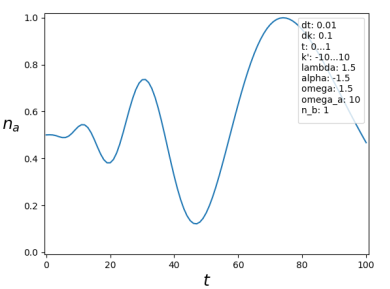
\includegraphics[width=0.65\linewidth]{pictures/result_first_1.png}
    \caption{Осциллирующее поведение}
    \label{fig:fr_oscillation}
\end{figure}

Такой результат сложно~объяснить с точки~зрения когнитивной психологии, поскольку экспериментов с таким
эффектом найти не удалось.
Результат моделирования приведенный на рисунке~\ref{fig:fr_oscillation} можно описать как "метание"
агента из одного выбора к другому, когда человеку через некоторое время кажется, что он сделал фатальную
ошибку в выборе, но такое объяснение, к сожалению, не удалось привести из-за отсутствия реальных
экспериментов.
Помимо необъяснимости полученного результата, приведенного на рисунке~\ref{fig:fr_oscillation}, стоит
отметить отсутствие комплексной плоскости на графике, поскольку присутствие комплексной составляющей
в результате моделирования дает предпосылки к ошибке вычисления, а это необходимо учитывать при моделировании.
Такой же результат без комплексной плоскости необходимо отметить на следующем графике (рисунок~\ref{fig:fr_next}).
\begin{figure}[h!]
    \centering
    \captionsetup{justification=centering}
    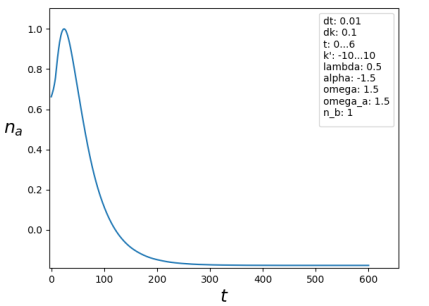
\includegraphics[width=0.7\linewidth]{pictures/result_first_2.png}
    \caption{Экспоненциальное затухание когнитивного возбуждения с пичком}
    \label{fig:fr_next}
\end{figure}

На~рисунке~\ref{fig:fr_next}~происходит~некоторое~временное возбуждение с последующим затуханием,~поведение
которого~также объясняется комплексным или отрицательным параметром плотности $g$.
В когнитивистике это поведение можно объяснить как ситуацию с отрицанием противоположной точки зрения.
Когда среда начинает воздействовать на сознание противоречивой информацией, вызывая у человека когнитивный
диссонанс, проявляющаяся ответной реакцией в виде пичка на графике, но через некоторое время ответная
реакция сознания индивида постепенно затухает, иначе говоря индивид переходит к состноянию среды.

Более правильным поведением является случай с параметром плотности $g = 1$, по причине отсутствия
комплексной составляющей в результатах модели, иначе говоря $n_{a} \in \mathbb{R}$.
Конечно, данное действие не является правильным с точки зрения вычислений, поскольку в таком случае
коммутатор в уравнении~\eqref{dynamic_comm} не равняется нулю, а это значит что оператор рождения и
уничтожения агента не коммутируют, чего не должно происходить.
Поведение при $g = 1$ показано на рисунке~\ref{fig:fr_real_g_15}.
\begin{figure}[h!]
    \centering
    \captionsetup{justification=centering}
    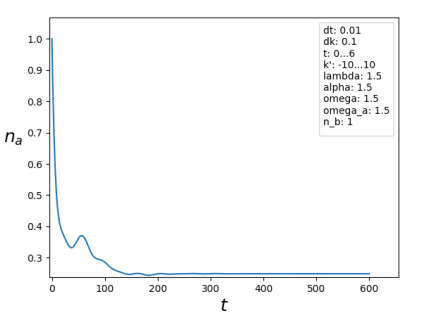
\includegraphics[width=0.7\linewidth]{pictures/result_first_4.png}
    \caption{Экспоненциальное затухание при вещественном значении параметра $g$}
    \label{fig:fr_real_g_15}
\end{figure}
Как видно из рисунка~\ref{fig:fr_real_g_15} его поведение схоже с марковской квантово-подобной моделью,
про которую было сказано ранее, приведенной в уравнении~\eqref{na_bagarello} и на рисунке~\ref{fig:at_baga}.
С точки зрения квантовой когнитивистики это поведение было описано ранее в других
работах~\citep{bagarello2015quantum,bagarello2018quantum}.

В залючении этой части необходимо уточнить причины проблемы присутствия комплексной составляющей в модели.
Проблема заключается не только в том, что параметр плотности $g$ вносит комплексную составляющую в оператор
принятия решения $n_{a} \in \mathbb{C}$, но и в том, что поскольку даже отнормировав основные уравнения
по $g$, из-за чего в коммутаторе~\eqref{dynamic_comm} он исчезает, отрицаельными или комплексными окажутся
другие параметры, так как необходимо соблюдать коммутационные соотношения.
Решением этой проблемы может быть поиск аналитического способа, но в данной работе этого сделать не удалось.
В таком случае необходимо найти приближенный вид аналитического решения, что может быть осуществимо.

%%%%%%%%%%%%%%%%%%%%%%%%%%%%%%%%%%%%%%%%%%%%%%%%%%%%%%%%%%%%%%%%%%%%%%%%%%%%%%%%%%%%%%%%%%%%%%%%%%%%
%%%%%%%%%%%%%%%%%%%%%%%%%%%%%%%%%%%%%%%%%%%%%%%%%%%%%%%%%%%%%%%%%%%%%%%%%%%%%%%%%%%%%%%%%%%%%%%%%%%%
\section{Второй способ моделирования}

Для приближенного аналитического решения необходимо найти численное решение уравнения для оператора
агента $a(t), a^{\dagger}(t)$.
В основу численного решения было взято нормированное по $g$ уравнение~\eqref{dotat_norm}, вывод которого
подробно приведен в приложении.
\begin{equation}\label{dotat_norm}
    \dot{a}(t) =
    -i \omega^{'}_{a} a(t)
    -i \lambda \int \frac{b(k)e^{-i \omega k t}}{\sqrt{k^{2} + \alpha^2}} dk
    -\frac{\lambda^{2} \pi}{\alpha} \int_{0}^{t} a(\tau) e^{- \alpha \omega (t - \tau)} d\tau
\end{equation}
Как видно из уравнения~\eqref{dotat_norm} в нем отсутствует параметр плотности, а это значит его
задавать не нужно.
Применяем итерационный метод решения для уравнения~\eqref{dotat_norm}, который имеет вид:
\begin{multline}
    a(t + \Delta t) =
    -i \omega^{'}_{a} a(t) \Delta t
    -i \lambda \int \frac{b(k)e^{-i \omega k t}}{\sqrt{k^{2} + \alpha^2}} dk \Delta t \\
    -\frac{\lambda^{2} \pi}{\alpha} \int_{0}^{t} a(\tau) e^{- \alpha \omega (t - \tau)} d\tau \Delta t
    - a(t)
\end{multline}
Все параметры в этом уравнении задаются случайным способом в диапазоне вещественных чисел кроме одного.
Этим параметром является оператор резервуара $b(k), b^{\dagger}(k)$, который задается в области
комплексных значений.
В ходе расчетов было выяснено, что большую зависимость оператор агента $a(t), a^{\dagger}(t)$ проявляет
в зависимости от оператора резервуара $b(k), b^{\dagger}(k)$, а это зачит необходимо продумать
приближенные значения этого параметра в итерационном методе решения.
Поскольку известно, что операторы рождения и уничтожения комплексно-сопряженные между собой, то значит
можно предположить отличия между оператором рождения и уничтожения только знаком комплексной составляющей.
Помимо этого, параметр $b(k), b^{\dagger}(k)$ не просто число, а некоторая зависимость от параметра $k$.
Такая зависимость может иметь большое количество вариантов, из которых выявить основные не получится.
Моделирование оператора рождения и уничтожения резервуара $b(k), b^{\dagger}(k)$ нетривиальная задача,
которая требует отдельного рассмотрения, но без него невозможны дальнейшие действия.
В таком случае оператор рождения и уничтожения для резервуара были приняты равными константе
$b(k) = b, b^{\dagger}(k) = b^{\dagger}$, при этом они должны быть комплексно-сопряженными.

После численного решения оператора рождения и уничтожения агента $a(t), a^{\dagger}(t)$ остается
вопрос о проверке результатов.
Проверка результатов может быть проведена с помощью коммутационных соотношений $[a(t), a^{\dagger}(t)] = 1$,
которые уже были показаны в данной работе.
Эти коммутационные соотношения работают только для $a(t), a^{\dagger}(t)$, но не для
$\dot{a}(t), \dot{a}^{\dagger}(t)$, поэтому нужно найти хотя бы приближенное аналитическое решение.
Хорошим показателем правильного моделирования является отсутствие комплексного составляющего в результате
получения оператора принятия решения $n_{a}$, но для данного метода решения этого можно не делать,
поскольку параметры задаются вещественными в начале моделирования.
Получив итерационным методом оператор рождения и уничтожения агента $a(t), a^{\dagger}(t)$, можно
перейти к численному результату оператора принятия решения $n_{a}$.
Результаты численного решения оператора принятия решения преведны в следующей части главы.

%%%%%%%%%%%%%%%%%%%%%%%%%%%%%%%%%%%%%%%%%%%%%%%%%%%%%%%%%%%%%%%%%%%%%%%%%%%%%%%%%%%%%%%%%%%%%%%%%%%%
%%%%%%%%%%%%%%%%%%%%%%%%%%%%%%%%%%%%%%%%%%%%%%%%%%%%%%%%%%%%%%%%%%%%%%%%%%%%%%%%%%%%%%%%%%%%%%%%%%%%
\section{Результаты вычисления вторым способом}

Для данного способа решения полученные данные оказались более правильными, поскольку комплексная составляющая
отсутствовала для всех результатов моделирования.
Результаты моделирования хорошо показывают проявление немарковского процесса, эффекта влияния "памяти"
на принятие решения, постепенный переход к равновесию в информационном резервуаре.
Разработанная модель очень просто сводится к результатам марковской квантово-подобной модели~\citep{bagarello2018quantum},
если задать степень влияния осцилляций на модель достаточно слабыми, а параметр $\alpha$ задать гораздо
больше чем в два раза частотной характеристики $\omega_{a}$, что как раз приведено на рисунке~\ref{fig:sr_mark}.
\begin{figure}[h!]
    \centering
    \captionsetup{justification=centering}
    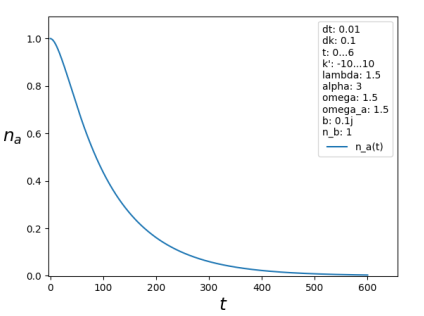
\includegraphics[width=0.7\linewidth]{pictures/result_second_1.png}
    \caption{Марковское приближение при малых осцилляциях резервуара и $\alpha = 3$}
    \label{fig:sr_mark}
\end{figure}

Для сравнения приведенного результата на рисунке~\ref{fig:sr_mark} с марковской квантово-подобной
моделью принятия решения можно обратиться к рисунку~\ref{fig:at_baga}.
Этот результат не представляет интереса в даннной работе, поскольку такие результаты обсуждались в других работах.
Другой случай показывает влияние немарковского процесса на поведение агента при воздействии резервуара,
который приведен на рисунке~\ref{fig:sr_nomark}.
\begin{figure}[h!]
    \centering
    \captionsetup{justification=centering}
    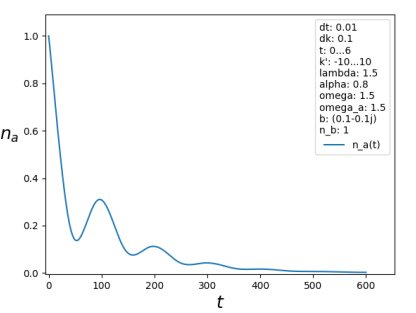
\includegraphics[width=0.7\linewidth]{pictures/result_second_2.png}
    \caption{Немарковское поведение при малых осцилляциях резервуара и $\alpha = 0.8$}
    \label{fig:sr_nomark}
\end{figure}

Как видно из рисунка~\ref{fig:sr_nomark} агент стремится к начальному решению через некоторое время
равному $t = 100, 200, 300$, происходят осциляции с затуханием.
Такое поведение, с точки зрения конитивистики, объясняется как "когнитивный шум" и наблюдается в
социальных сетях при воздействии информационной среды сообщества на участника этого сообщества.
Как видно из рисунка~\ref{fig:sr_mark} и рисунка~\ref{fig:sr_nomark} немарковский процесс может
переходить в марковский, в случае малых величин оператора рождения(уничтожения) резервуара $b, b^{\dagger}$
и параметра $\alpha$ больше частотной характеристики агента $\omega_{a}$.
Было обнаружено, что при уменьшении параметра $\alpha$ относительно частотной характеристики $\omega_{a}$,
увеличивается частота осциляций модели, что в данном случае наблюдается на рисунке~\ref{fig:sr_more_oscillation}.
\newpage
\begin{figure}[h!]
    \centering
    \captionsetup{justification=centering}
    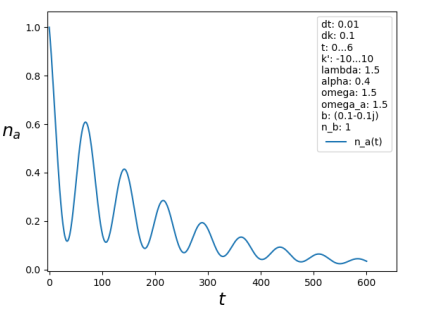
\includegraphics[width=0.7\linewidth]{pictures/result_second_3.png}
    \caption{Немарковское поведение при малых осцилляциях резервуара и $\alpha = 0.4$}
    \label{fig:sr_more_oscillation}
\end{figure}
Необходимо отметить зависимость диапазона моделирования от величины модуля оператора рождения(уничтожения)
резевуара $\arrowvert b \arrowvert, \arrowvert b^{\dagger} \arrowvert$.
Поскольку диапазон принятия решения находится в пределах от 0 до 1, то и параметры модели должны быть
подобраны таким образом, чтобы в результате соответсвовать этим ограничениям.
Поэтому сумма модулей оператора рождения и уничтожения резервуара не должны превышать 1, иначе говоря
сумма радиусов их векторов на комплексной плоскости не должны первышать 1.
На рисунке~\ref{fig:sr_more_oscillation} можно заметить, что нижние полупериоды осцилляций модели достигают
минимума постепенно, по закону гауссовой функции.
Это поведение можно наблюдать в физике при изучении степени пространственной когерентности реальных
лазерных источников в интерверометре Юнга, когда темные полосы интерференционной картины "засвечены"
нескоррелированными фотонами.
Такое поведение моделируется если сумма действительной части оператора рождения и уничтожения резервуара
близка по сумме к 1.
Более наглядное представление этого поведения представлено на рисунке~\ref{fig:sr_gauss}.
\begin{figure}[h!]
    \centering
    \captionsetup{justification=centering}
    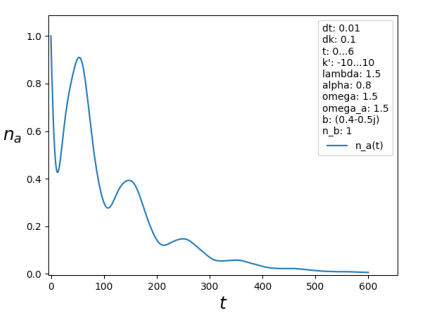
\includegraphics[width=0.7\linewidth]{pictures/result_second_4.png}
    \caption{Немарковское поведение с возвышенными нижними полупериодами осцилляций}
    \label{fig:sr_gauss}
\end{figure}
Песледний вопрос в этой части касается приближенного аналитического вида модели принятия решения.
Для решения вопроса необходимо описать основные уравнения, которые будут составлять характер модели.
Первое что необходимо отметить, это присутствие осцилляций, характер которых может описать уравнение
косинуса.
Поскольку косинус находится в пределе от -1 до 1, то его значения нужно увеличить на единицу.
Осцилляции в модели со временем затухают и их характер затухания необходимо подбирать.
Для уравнения затухания было выбрано уравнение экспоненты в отрицательной степени, которая составляет
проезведение с уравнением косинуса.
В вышеприведенных результатах поведение агента стремится к покою(к 0) и это значит присутствие экспоненты
в знаменателе для всего полученного аналитического решения.
Окончательный результат этой приближенной модели представлен следующим образом:
\begin{equation}
    f(t) = \frac{cos(tx - y)*e^{-tz} + 1}{e^{t}},
\end{equation}
где $x$ - параметр частоты, $y$ - параметр сдвига, $z$ - параметр затухания осцилляций, $t$ - время.
Для демонстрации результатов поиска приближенного решения оператора принятия решения следует привести
уравнения с подобраными параметрами.
Первое уравнение имеет следующий вид:
\begin{equation}
    f(t) = \frac{cos(10*t/1.645 - 10)*e^{-t*0.3} + 1}{e^{t}},
\end{equation}
и его результат с приведенным немарковским поведением модели при сильных осциллциях и их "сильных" минимумов~\ref{fig:sr_proba_1}.
\begin{figure}[h!]
    \centering
    \captionsetup{justification=centering}
    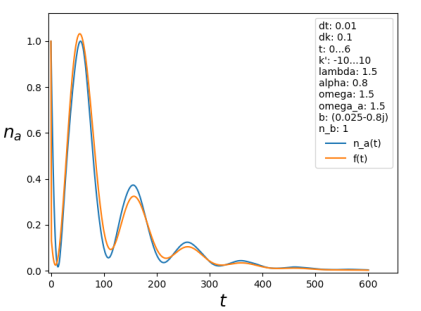
\includegraphics[width=0.7\linewidth]{pictures/result_second_5.png}
    \caption{Поведение модели и приблеженного аналитического решения}
    \label{fig:sr_proba_1}
\end{figure}
Второе уравнение имеет следующий вид:
\begin{equation}
    f(t) = \frac{cos(10*t/1.645 - 9.5)*e^{-t*0.8} + 1}{e^{t}},
\end{equation}
где его результат с вышеприведенным поведением приведен на следующем рисунке~\ref{fig:sr_proba_2}.
\newpage
\begin{figure}[h!]
    \centering
    \captionsetup{justification=centering}
    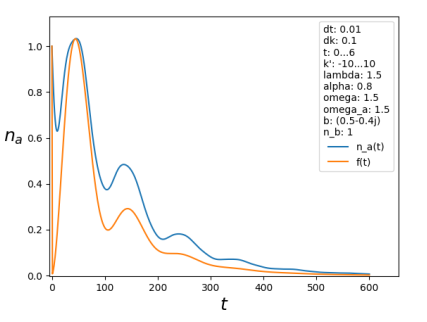
\includegraphics[width=0.7\linewidth]{pictures/result_second_6.png}
    \caption{Поведение модели и приблеженного аналитического решения с другими параметрами}
    \label{fig:sr_proba_2}
\end{figure}

Коммутационное соотношение из приближенного уравнения взять не получится, поскольку отсутствует
оператор рождения(уничтожения) в слагаемых.
Но основная задача данной работы решена, поскольку была получена модель, описывающая эмпирические
данные в социальных сетях.